\chapter{Introduction}

What was/is the purpose of this thesis? Why did we develop these computational simulations? Really, we need a goal!

In this thesis, a lattice Monte Carlo approach was used to simulate diffusion. Also used a finite difference method to simulate diffusion. Both problems were boundary-value problems.

We also performed an analysis: MSD, mean position, etc.?? Analysis is kind of empty!

\section{Background}
	Overall overview to thesis? What kind of an overview? Or just a general background to some main concepts needed or used in this thesis? How does this compare with the abstract?
	
\section{Diffusion}
Say something general 

\section{Monte Carlo}


\section{Finite Difference Solution of the Diffusion Equation}
This was done is 1D and 2D.

\section{Simple Cell Model}



%\section{A sample introduction}
%
%This is just an example, but I wanted to show you some common things to do with Latex.
%
%\subsection{A subsection example}
%
%For of all, here's an equation -- it's the NFW formula, given by \citet{nfw95}, and looks like
%\begin{equation}
%	\label{eq:nfw}
%	\rho(r) = \frac{\rho_s}{r / r_s (1 + r / r_s)^2},
%\end{equation}
%where $\rho_s$ and $r_s$ are a characteristic density and scale radius, respectively.
%
%Now, I can reference that equation later, since it's labelled properly; it's equation (\ref{eq:nfw}).  Notice that I cited a paper above; I could do that in a different way like this \citep{nfw95}.
%
%Just one other quick thing:  figures.  There's one below, and again it's properly labelled.  It's Figure \ref{fig:intro_density}.
%
%\begin{figure}
%\begin{center}
%	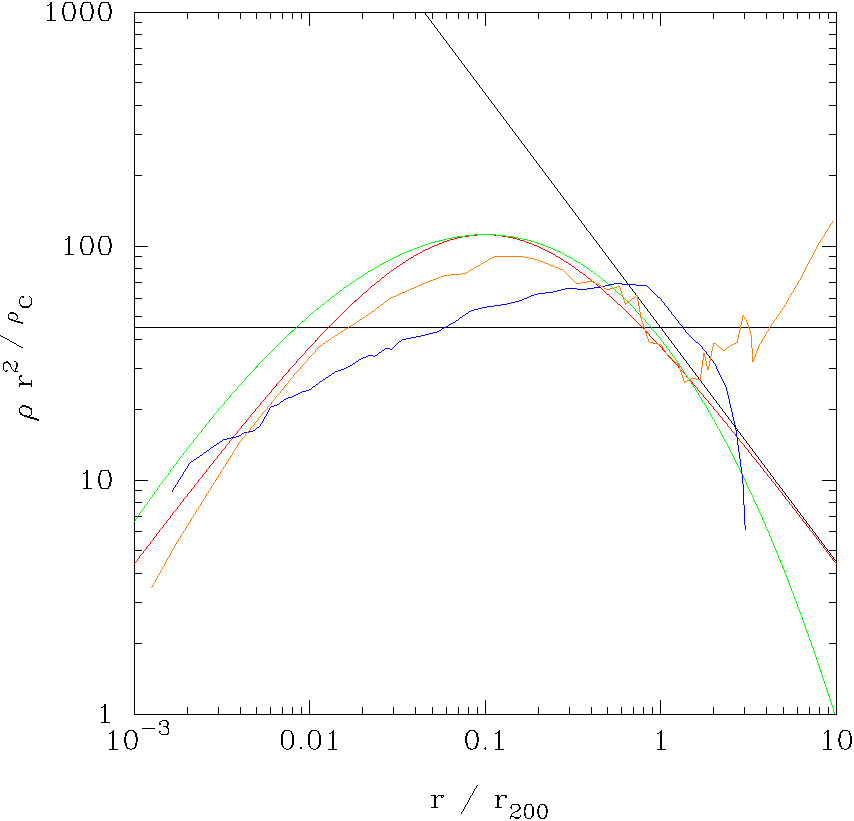
\includegraphics[scale=0.8]{intro_density.pdf}
%\end{center}
%	\caption[Density profiles of various models]{Density profiles, shown as $\rho r^2$ to better highlight the differences, of various models.  }
%	\label{fig:intro_density}
%\end{figure}